\documentclass[12pt,a4paper]{article}

\usepackage[utf8]{inputenc}
\usepackage[T1]{fontenc}
\usepackage[brazil]{babel}
\usepackage{lmodern}
\usepackage[a4paper,margin=2.5cm]{geometry}
\usepackage{amsmath,amssymb}
\usepackage{graphicx}
\usepackage{booktabs}
\usepackage{multirow}
\usepackage{float}
\usepackage{caption}
\usepackage{xcolor}
\usepackage{listings}
\usepackage[hidelinks]{hyperref}

\definecolor{codebg}{RGB}{248,248,248}
\definecolor{codecomment}{RGB}{0,110,0}
\definecolor{codekw}{RGB}{0,0,160}
\definecolor{codestr}{RGB}{160,40,40}

\lstset{
  language=Python,
  basicstyle=\ttfamily\footnotesize,
  backgroundcolor=\color{codebg},
  keywordstyle=\color{codekw}\bfseries,
  commentstyle=\color{codecomment}\itshape,
  stringstyle=\color{codestr},
  numbers=left,
  numberstyle=\tiny\color{gray},
  frame=single,
  breaklines=true,
  showstringspaces=false,
  tabsize=4,
  inputencoding=utf8,
  extendedchars=true,
  literate=
    {á}{{\'a}}1 {à}{{\`a}}1 {ã}{{\~a}}1 {â}{{\^a}}1
    {é}{{\'e}}1 {ê}{{\^e}}1 {í}{{\'i}}1
    {ó}{{\'o}}1 {õ}{{\~o}}1 {ô}{{\^o}}1
    {ú}{{\'u}}1 {ç}{{\c{c}}}1
    {Á}{{\'A}}1 {É}{{\'E}}1 {Í}{{\'I}}1 {Ó}{{\'O}}1 {Ú}{{\'U}}1 {Ç}{{\c{C}}}1
}

% Link do repositório do código
\newcommand{\repositorio}{\url{https://github.com/juliaPamplona/teia-laboratorios/tree/main/lab3}}

\newcommand{\setosa}{\emph{setosa}}
\newcommand{\versicolor}{\emph{versicolor}}
\newcommand{\virginica}{\emph{virginica}}

\begin{document}

%=====================================================================
% Capa
%=====================================================================
\begin{titlepage}
\centering

\includegraphics[width=0.35\textwidth]{figuras/logo_uepb.png}\\[1.5em]
{\large \textsc{Universidade Estadual da Paraíba}}\\[0.3em]
{\normalsize Disciplina: Tópicos Especiais em Inteligência Artificial}\\[0.3em]
{\normalsize Prof. Robson Pequeno de Sousa}

\vfill

{\LARGE \textbf{Perceptron com regra delta e métricas de qualidade de classificadores aplicados à base Iris}}\\[1em]
{\large Relatório do Laboratório 03 --- Regra delta (PR41) e métricas de qualidade em aprendizado de máquina (PR51)}

\vfill

{\large Júlia Pamplona}

\vfill

{\large Novembro de 2026}
\end{titlepage}

%=====================================================================
% Resumo
%=====================================================================
\begin{abstract}
Este relatório descreve duas etapas implementadas em Python, sem bibliotecas de aprendizado de máquina. Na primeira, o perceptron com regra delta foi treinado nos três pares de espécies da base Iris (70\% para treinamento e 30\% para teste) e nas tabelas verdade OR, AND e XOR, com o acompanhamento do erro quadrático médio (EQM) por época. O EQM estabilizou em todos os casos; a separação sem erros foi obtida nos pares com a \setosa{} (quatro atributos) e nas tabelas OR e AND, mas não no par \virginica{}~$\times$~\versicolor{} nem no XOR, que não são linearmente separáveis. Na segunda etapa, foram implementadas as métricas de qualidade da aula PR51 --- acerto global, acurácias do produtor e do usuário, coeficientes Kappa e Tau com suas variâncias, teste de significância $Z$, $F_1$, $F_2$ e coeficiente de Matthews --- e usadas para comparar cinco classificadores das três classes da Iris: distância mínima, máximo da função de decisão, superfície de decisão um contra todos, perceptron e regra delta. A superfície de decisão obteve o maior Kappa (0,867), seguida do perceptron (0,833), da distância mínima (0,800) e da regra delta (0,733), mas nenhum par de classificadores difere significativamente ao nível de 5\%, o que se explica pelas apenas 45 amostras de teste. Por fim, foram resolvidos os exercícios da aula, incluindo o desafio obrigatório, em que os classificadores A e B (Kappa 0,847 e 0,806) também não diferem a 5\% ($Z = 1{,}59$, $p = 0{,}11$).

\vspace{1em}
\noindent\textbf{Palavras-chave:} regra delta; matriz de confusão; coeficiente Kappa; coeficiente Tau; coeficiente de Matthews; F-score; teste de significância; base Iris.
\end{abstract}
\thispagestyle{empty}
\newpage

%=====================================================================
% Sumário
%=====================================================================
\tableofcontents
\thispagestyle{empty}
\newpage

%=====================================================================
\section{Introdução}
%=====================================================================

Nos laboratórios anteriores, a base Iris foi classificada pela distância mínima e pelas funções de decisão calculadas a partir dos protótipos das classes (Laboratório~01) e pelo algoritmo perceptron (Laboratório~02). Em todos eles o desempenho foi resumido pela acurácia, isto é, pela fração de amostras classificadas corretamente. Esta medida, porém, não diz quais classes são confundidas entre si, não desconta os acertos que ocorreriam por acaso e não permite decidir se a diferença entre dois classificadores é real ou fruto da amostra usada no teste.

Este laboratório tem duas partes. A primeira implementa o perceptron com regra delta (aula PR41), que, diferentemente do perceptron simples, corrige os pesos a cada padrão na proporção do erro contínuo e por isso sempre estabiliza o EQM. A segunda implementa as métricas de qualidade da aula PR51 e as aplica aos classificadores vistos até aqui, agora para as três classes da Iris ao mesmo tempo. Os objetivos são:
\begin{enumerate}
  \item Classificar as três classes da Iris com o classificador de distância mínima, o de máximo da função de decisão, a superfície de decisão na estratégia um contra todos, o perceptron e o perceptron com regra delta, e determinar, para cada um:
  \begin{enumerate}
    \item o acerto global;
    \item a acurácia do produtor;
    \item a acurácia do usuário;
    \item o coeficiente Kappa;
    \item o coeficiente Tau;
    \item o coeficiente de Matthews para o problema de duas classes;
    \item a medida $F_b$, com $b = 1$ e $b = 2$, para o problema de duas classes.
  \end{enumerate}
  \item Verificar, com o teste de significância do Kappa, se a superfície de decisão e o perceptron diferem, e comparar o perceptron com regra delta e o perceptron pelos testes de Kappa e Tau.
  \item Resolver os exercícios definidos na aula PR51.
\end{enumerate}

%=====================================================================
\section{Fundamentação teórica}\label{sec:teoria}
%=====================================================================

\subsection{Perceptron com regra delta}\label{sec:regra_delta}

Com vetores aumentados $\mathbf{x} = (x_1, \dots, x_n, 1)^t$ e $\mathbf{w} = (w_1, \dots, w_n, w_0)^t$, a função discriminante linear é $g(\mathbf{x}) = \mathbf{w}^t\mathbf{x}$, e o padrão é atribuído à classe $\omega_1$ (resposta $+1$) se $g(\mathbf{x}) > 0$ e à classe $\omega_2$ (resposta $-1$) caso contrário. Sendo $r_i \in \{+1, -1\}$ a resposta desejada, o erro quadrático total e o EQM são
\begin{equation}
  E(\mathbf{w}) = \frac{1}{2}\sum_{i=1}^{n} \left(r_i - \mathbf{w}^t\mathbf{x}_i\right)^2,
  \qquad \text{EQM} = \frac{E(\mathbf{w})}{n}.
  \label{eq:eqm}
\end{equation}
A regra delta minimiza $E(\mathbf{w})$ por gradiente descendente, corrigindo o vetor peso a cada padrão apresentado:
\begin{equation}
  \mathbf{w}(k+1) = \mathbf{w}(k) + \alpha\left[r(k) - \mathbf{w}^t(k)\,\mathbf{x}(k)\right]\mathbf{x}(k),
  \qquad 0{,}1 < \alpha < 1{,}0.
  \label{eq:regra_delta}
\end{equation}
O perceptron simples só corrige os pesos quando erra a classificação; a regra delta corrige sempre, na proporção do erro $r - \mathbf{w}^t\mathbf{x}$. Por isso o EQM converge para um mínimo mesmo quando as classes não são linearmente separáveis. Esse mínimo, contudo, é o do erro quadrático, e não o do número de erros de classificação: a solução pode deixar padrões do lado errado mesmo quando existe uma reta que separa as classes.

\subsection{Matriz de confusão}

Para $C$ classes, a matriz de confusão cruza a classificação (linhas) com a referência (colunas), como na Tabela~\ref{tab:matriz_geral}. O elemento $a_{ij}$ é o número de exemplos atribuídos à classe $\omega_i$ que pertenciam à classe $\omega_j$; $a_{i+}$ e $a_{+i}$ são os totais da linha e da coluna $i$, e $m$ é o total de exemplos. A diagonal contém os acertos.

\begin{table}[H]
\centering
\caption{Matriz de confusão para $C$ classes (linhas: classificação; colunas: referência).}
\label{tab:matriz_geral}
\begin{tabular}{cc|cccc|c}
\toprule
 & & \multicolumn{4}{c|}{Referência} & \\
 & & $\omega_1$ & $\omega_2$ & $\cdots$ & $\omega_C$ & Total \\
\midrule
\multirow{4}{*}{\rotatebox{90}{Classificação}}
 & $\omega_1$ & $a_{11}$ & $a_{12}$ & $\cdots$ & $a_{1C}$ & $a_{1+}$ \\
 & $\omega_2$ & $a_{21}$ & $a_{22}$ & $\cdots$ & $a_{2C}$ & $a_{2+}$ \\
 & $\vdots$   & $\vdots$ & $\vdots$ & $\ddots$ & $\vdots$ & $\vdots$ \\
 & $\omega_C$ & $a_{C1}$ & $a_{C2}$ & $\cdots$ & $a_{CC}$ & $a_{C+}$ \\
\midrule
 & Total & $a_{+1}$ & $a_{+2}$ & $\cdots$ & $a_{+C}$ & $m$ \\
\bottomrule
\end{tabular}
\end{table}

\subsection{Acerto global e acurácias do produtor e do usuário}

O acerto global é a fração de predições corretas:
\begin{equation}
  A_g = \frac{1}{m}\sum_{i=1}^{C} a_{ii}.
  \label{eq:ag}
\end{equation}
A avaliação por classe é feita pela acurácia do produtor, probabilidade de uma observação da classe $\omega_i$ ser classificada corretamente (sensibilidade), e pela acurácia do usuário, probabilidade de uma observação classificada como $\omega_i$ pertencer de fato a essa classe (precisão, ou valor preditivo positivo):
\begin{equation}
  A_{pi} = \frac{a_{ii}}{a_{+i}}, \qquad A_{ui} = \frac{a_{ii}}{a_{i+}}.
  \label{eq:ap_au}
\end{equation}

\subsection{Coeficiente Kappa e sua variância}

O coeficiente Kappa mede a concordância entre a predição e a referência descontando a concordância esperada por acaso. Sendo $A_a$ o acerto casual,
\begin{equation}
  K = \frac{A_g - A_a}{1 - A_a}, \qquad
  A_a = \frac{1}{m^2}\sum_{i=1}^{C} a_{i+}\,a_{+i}, \qquad K \in \left]-\infty, 1\right].
  \label{eq:kappa}
\end{equation}
$K = 1$ indica concordância perfeita e $K = 0$, concordância igual à do acaso. A interpretação usual é a de Landis e Koch~\cite{landis}: fraca ($K \le 0{,}20$), razoável ($0{,}21$--$0{,}40$), moderada ($0{,}41$--$0{,}60$), substancial ($0{,}61$--$0{,}80$) e quase perfeita ($0{,}81$--$1{,}00$).

A variância do Kappa (Congalton e Green~\cite{congalton}) é
\begin{equation}
  \sigma_K^2 = \frac{1}{m}\left[
    \frac{\phi_1(1-\phi_1)}{(1-\phi_2)^2}
  + \frac{2(1-\phi_1)(2\phi_1\phi_2-\phi_3)}{(1-\phi_2)^3}
  + \frac{(1-\phi_1)^2(\phi_4-4\phi_2^2)}{(1-\phi_2)^4}
  \right],
  \label{eq:var_kappa}
\end{equation}
com
\begin{equation}
  \phi_1 = A_g,\quad \phi_2 = A_a,\quad
  \phi_3 = \frac{1}{m^2}\sum_{i=1}^{C} a_{ii}\,(a_{i+} + a_{+i}),\quad
  \phi_4 = \frac{1}{m^3}\sum_{i=1}^{C}\sum_{j=1}^{C} a_{ij}\,(a_{j+} + a_{+i})^2.
  \label{eq:phis}
\end{equation}

\subsection{Coeficiente Tau e sua variância}

O coeficiente Tau supõe que os acertos casuais se distribuem uniformemente entre as $C$ classes, ou seja, troca $A_a$ por $1/C$:
\begin{equation}
  \tau = \frac{A_g - \frac{1}{C}}{1 - \frac{1}{C}}, \qquad
  \sigma_\tau^2 = \frac{1}{m}\,\frac{A_g(1-A_g)}{\left(1-\frac{1}{C}\right)^2}.
  \label{eq:tau}
\end{equation}

\subsection{Teste de significância}\label{sec:teste}

Para decidir se dois classificadores diferem, testam-se as hipóteses $H_0$: não há diferença entre os coeficientes, e $H_1$: há diferença, com a estatística
\begin{equation}
  Z = \frac{k_1 - k_2}{\sqrt{\sigma_1^2 + \sigma_2^2}} \sim N(0, 1),
  \label{eq:z}
\end{equation}
em que $k$ é o Kappa ou o Tau de cada classificador e $\sigma^2$ a variância correspondente. Fixado $\alpha$, rejeita-se $H_0$ se $|Z| > Z_{1-\alpha/2}$; para $\alpha = 5\%$, $Z_{0{,}975} = 1{,}96$. O p-valor é $p = P(|Z| > |z|)$, a probabilidade de observar uma diferença pelo menos tão grande quanto a obtida se $H_0$ fosse verdadeira; $p < 0{,}05$ indica diferença significativa.

\subsection{Métricas para duas classes}\label{sec:binarias}

Num problema de duas classes, em que uma indica a ocorrência de uma condição, a matriz de confusão se reduz a verdadeiros positivos (VP), falsos positivos (FP), falsos negativos (FN) e verdadeiros negativos (VN), e as métricas são
\begin{equation}
  S_e = R_e = \frac{VP}{VP + FN},\quad
  E_s = \frac{VN}{VN + FP},\quad
  P_r = \frac{VP}{VP + FP},\quad
  A_c = \frac{VP + VN}{VP + FP + FN + VN},
  \label{eq:binarias}
\end{equation}
isto é, sensibilidade (revocação), especificidade, precisão e acurácia. A medida $F_b$ é a média harmônica ponderada de precisão e revocação, e o coeficiente de Matthews (MCC) usa os quatro valores da matriz:
\begin{equation}
  F_b = (1 + b^2)\,\frac{P_r R_e}{b^2 P_r + R_e}, \qquad
  \text{MCC} = \frac{VP\cdot VN - FP\cdot FN}{\sqrt{(VP+FP)(VP+FN)(VN+FP)(VN+FN)}}.
  \label{eq:fb_mcc}
\end{equation}
Com $b = 1$, precisão e revocação têm o mesmo peso; com $b = 2$, a revocação pesa mais, o que é preferível quando o falso negativo é o erro mais grave. O $F_b$ não usa os VN e pode enganar quando as classes estão desbalanceadas; o MCC, limitado a $[-1, 1]$, vale 1 para predições totalmente concordantes, $-1$ para totalmente discordantes e fica próximo de zero para concordância aleatória.

\paragraph{Observações sobre as fórmulas dos slides.} Duas diferenças em relação aos slides da aula foram adotadas e conferidas:
\begin{itemize}
  \item no slide do $F_b$ o numerador aparece como $(1 + b)$; a definição usual~\cite{sokolova} é $(1 + b^2)$. As duas coincidem para $b = 1$, mas só $(1 + b^2)$ dá $F_2 = 1$ quando $P_r = R_e = 1$;
  \item no slide da variância do Kappa, o termo $(a_{j+} + a_{+i})$ de $\phi_4$ aparece sem o expoente 2, que está presente na fórmula original~\cite{congalton}. A versão com o quadrado foi validada por simulação (Seção~\ref{sec:validacao}).
\end{itemize}

%=====================================================================
\section{Base de dados}
%=====================================================================

A base Iris (arquivo \texttt{Iris data.xls}) contém 150 amostras, 50 de cada espécie: \setosa{}, \versicolor{} e \virginica{}. Cada amostra é descrita pelo vetor de características $\mathbf{x} = (x_1, x_2, x_3, x_4)^t$ da Tabela~\ref{tab:atributos}.

\begin{table}[H]
\centering
\caption{Atributos da base Iris na ordem do arquivo.}
\label{tab:atributos}
\begin{tabular}{cll}
\toprule
Atributo & Coluna & Descrição \\
\midrule
$x_1$ & \texttt{Sepal length} & comprimento da sépala (cm) \\
$x_2$ & \texttt{Sepal width}  & largura da sépala (cm) \\
$x_3$ & \texttt{Petal length} & comprimento da pétala (cm) \\
$x_4$ & \texttt{Petal width}  & largura da pétala (cm) \\
\bottomrule
\end{tabular}
\end{table}

%=====================================================================
\section{Metodologia e implementação}
%=====================================================================

O código foi escrito em Python, usando apenas \texttt{pandas} (leitura da planilha), \texttt{numpy} (álgebra vetorial) e \texttt{matplotlib} (gráficos). A divisão da amostra, o treinamento, a classificação, a matriz de confusão, as métricas e o p-valor (pela função erro complementar, \texttt{math.erfc}) foram implementados manualmente. O código-fonte e as figuras estão disponíveis no repositório \repositorio.

\subsection{Organização do sistema}

\begin{table}[H]
\centering
\caption{Módulos do Laboratório 03.}
\label{tab:modulos}
\begin{tabular}{lp{10.5cm}}
\toprule
Arquivo & Responsabilidade \\
\midrule
\texttt{regra\_delta.py}       & regra delta, EQM, classificação, teste de separabilidade e critério de convergência \\
\texttt{visualizacao.py}       & impressões no terminal e gráficos da Parte I \\
\texttt{lab3\_regraDelta.py}   & Parte I: pares da Iris e tabelas verdade com a regra delta \\
\texttt{metricas.py}           & matriz de confusão e todas as métricas da PR51, com autoteste pelos slides \\
\texttt{classificadores.py}    & os cinco classificadores para as três classes \\
\texttt{lab3\_metricas.py}     & Parte II: questões 1 e 2 \\
\texttt{exercicios\_pr51.py}   & Parte III: exercícios da aula PR51 \\
\bottomrule
\end{tabular}
\end{table}

\subsection{Divisão 70\% / 30\% e padronização}

A divisão é estratificada: as 50 amostras de cada espécie são embaralhadas (semente 42) e separadas em 35 para treinamento e 15 para teste, totalizando 105 e 45 amostras. A mesma divisão é usada nas duas partes. Nos perceptrons, os atributos são padronizados (\emph{z-score}) com a média e o desvio padrão do treinamento, para que todos fiquem na mesma escala e o mesmo $\alpha$ possa ser usado em todos os problemas. Os classificadores baseados em protótipos usam os atributos originais, como no Laboratório~01.

\subsection{Treinamento com a regra delta}

A Eq.~\eqref{eq:regra_delta} foi implementada com $\alpha = 0{,}2$, pesos iniciais nulos e apresentação dos padrões na ordem do conjunto de treinamento. O treinamento para quando $|\text{EQM}(k) - \text{EQM}(k-1)| < 10^{-8}$ ou após 1000 épocas.

\begin{lstlisting}[title=\texttt{regra\_delta.py} --- laço de treinamento]
for epoca in range(1, max_epocas + 1):

    for x, r in zip(X_aumentado, respostas):
        # REGRA DELTA: w(k+1) = w(k) + alpha [r - w^T x] x
        erro = r - w @ x
        w = w + alpha * erro * x

    historico_eqm.append(calcular_eqm(X_aumentado, respostas, w))
    historico_erros.append(
        int(np.sum(classificar(X_aumentado, w) != respostas))
    )

    if abs(historico_eqm[-2] - historico_eqm[-1]) < tolerancia:
        eqm_estabilizou = True
        break
\end{lstlisting}

Como ``convergir'' pode significar tanto a estabilização do EQM quanto a separação sem erros, o código mede as duas coisas, e o veredito ``converge'' exige ambas. A separabilidade linear do conjunto de treinamento é verificada à parte com o perceptron simples, que só termina sem erros quando as classes são separáveis.

\subsection{Classificadores para as três classes}\label{sec:classificadores}

Os cinco classificadores comparados na Parte II estão em \texttt{classificadores.py}:
\begin{enumerate}
  \item \textbf{Distância mínima:} o protótipo $\mathbf{m}_j$ é a média das amostras de treinamento da classe $\omega_j$, e $\mathbf{x}$ é atribuído à classe de menor $D_j(\mathbf{x}) = \|\mathbf{x} - \mathbf{m}_j\|$.
  \item \textbf{Máximo da função de decisão:} $d_j(\mathbf{x}) = \mathbf{x}^t\mathbf{m}_j - \frac{1}{2}\mathbf{m}_j^t\mathbf{m}_j$, e $\mathbf{x}$ é atribuído à classe de maior $d_j(\mathbf{x})$. Como $D_j^2 = \mathbf{x}^t\mathbf{x} - 2d_j(\mathbf{x})$ e $\mathbf{x}^t\mathbf{x}$ é igual para todas as classes, as predições coincidem com as da distância mínima.
  \item \textbf{Superfície de decisão um contra todos:} para cada classe $\omega_i$, constrói-se a superfície do Laboratório~01 entre o protótipo $\mathbf{m}_i$ e o protótipo do ``resto'', $\mathbf{m}_r$, média das amostras das outras duas classes:
  \begin{equation}
    d_i(\mathbf{x}) = (\mathbf{m}_i - \mathbf{m}_r)^t\mathbf{x} - \tfrac{1}{2}(\mathbf{m}_i - \mathbf{m}_r)^t(\mathbf{m}_i + \mathbf{m}_r).
    \label{eq:sup_ova}
  \end{equation}
  $d_i(\mathbf{x}) > 0$ indica a classe $\omega_i$. Quando mais de uma superfície, ou nenhuma, responde positivo, $\mathbf{x}$ é atribuído à classe de maior $d_i(\mathbf{x})$.
  \item \textbf{Perceptron um contra todos:} três perceptrons simples, cada um com resposta $+1$ para a sua classe e $-1$ para as demais, com incremento de correção $c = 1$ e limite de 1000 épocas. $\mathbf{x}$ é atribuído à classe de maior $g_i(\mathbf{x}) = \mathbf{w}_i^t\mathbf{x}$.
  \item \textbf{Regra delta um contra todos:} igual ao anterior, com cada $\mathbf{w}_i$ treinado pela regra delta.
\end{enumerate}
Nos dois perceptrons, cada $\mathbf{w}_i$ é dividido pela norma de $(w_1, \dots, w_n)$, de modo que $g_i(\mathbf{x})$ passa a ser a distância com sinal de $\mathbf{x}$ ao hiperplano $i$ e os três valores podem ser comparados entre si.

\begin{lstlisting}[title=\texttt{classificadores.py} --- superfície de decisão um contra todos]
def superficie_um_contra_todos(X_treino, y_treino, classes):
    W = []
    for c in classes:
        m_i = X_treino[y_treino == c].mean(axis=0)
        m_r = X_treino[y_treino != c].mean(axis=0)
        w = m_i - m_r
        w0 = -0.5 * np.dot(m_i - m_r, m_i + m_r)
        W.append(np.r_[w, w0])
    W = np.array(W)

    def prever(X):
        d = aumentar(X) @ W.T
        return np.asarray(classes)[np.argmax(d, axis=1)]

    return prever, {"W": W}
\end{lstlisting}

\subsection{Métricas}

A matriz de confusão segue a convenção da aula: linhas para a predição e colunas para a referência. As métricas multiclasse vêm diretamente das Eqs.~\eqref{eq:ag} a~\eqref{eq:tau}. A variância do Kappa ficou assim:

\begin{lstlisting}[title=\texttt{metricas.py} --- variância do Kappa]
def variancia_kappa(mc):
    mc = np.asarray(mc, dtype=float)
    m = mc.sum()
    linhas = mc.sum(axis=1)   # a_i+
    colunas = mc.sum(axis=0)  # a_+i

    phi1 = acerto_global(mc)
    phi2 = acerto_casual(mc)
    phi3 = np.sum(np.diag(mc) * (linhas + colunas)) / m ** 2
    phi4 = sum(
        mc[i, j] * (linhas[j] + colunas[i]) ** 2
        for i in range(len(mc))
        for j in range(len(mc))
    ) / m ** 3

    termo1 = phi1 * (1 - phi1) / (1 - phi2) ** 2
    termo2 = 2 * (1 - phi1) * (2 * phi1 * phi2 - phi3) / (1 - phi2) ** 3
    termo3 = (1 - phi1) ** 2 * (phi4 - 4 * phi2 ** 2) / (1 - phi2) ** 4

    return (termo1 + termo2 + termo3) / m
\end{lstlisting}

O MCC e o $F_b$ se aplicam a duas classes. Na Iris, cada matriz $3 \times 3$ foi reduzida a três problemas ``classe $i$ $\times$ resto'', com
\begin{equation}
  VP = a_{ii},\quad FP = a_{i+} - a_{ii},\quad FN = a_{+i} - a_{ii},\quad VN = m - VP - FP - FN.
  \label{eq:reducao}
\end{equation}

\subsection{Validação da implementação}\label{sec:validacao}

O módulo \texttt{metricas.py} tem um autoteste que reproduz a acurácia global do slide do RT-PCR (95,5\%) e o Kappa do slide dos radiologistas (0,776, arredondado para 0,78 na aula), além de casos extremos (concordância perfeita, $\text{MCC} = \pm 1$) e do p-valor de $Z = 1{,}96$ ($p = 0{,}05$). A variância do Kappa foi conferida por simulação: sorteando 40\,000 matrizes multinomiais com as proporções da classificação A do desafio (Seção~\ref{sec:desafio}), a variância dos Kappas obtidos foi 0,000297, contra 0,000295 da Eq.~\eqref{eq:var_kappa} com o quadrado em $\phi_4$.

%=====================================================================
\section{Parte I --- Resultados da regra delta}\label{sec:parte1}
%=====================================================================

\subsection{Pares de classes da base Iris}

A Tabela~\ref{tab:regra_delta} resume os experimentos. Com os quatro atributos, os pares com a \setosa{} convergem: o EQM estabiliza num valor baixo e o treinamento termina sem erros, com 100\% de acerto no teste. No par \virginica{}~$\times$~\versicolor{} o EQM também estabiliza, mas num patamar mais alto (Figura~\ref{fig:mse_iris}), e restam 3 erros no treinamento: as classes não são linearmente separáveis.

\begin{table}[H]
\centering
\caption{Perceptron com regra delta nos pares da Iris e nas tabelas verdade.}
\label{tab:regra_delta}
\small
\begin{tabular}{lrrrrcc}
\toprule
Experimento & Épocas & EQM final & Erros treino & Acurácia teste & Separável & Converge \\
\midrule
\setosa{} $\times$ \virginica{} (4 atrib.)         & 30 & 0,0110 & 0  & 100,00\% & sim & sim \\
\setosa{} $\times$ \versicolor{} (4 atrib.)        & 40 & 0,0364 & 0  & 100,00\% & sim & sim \\
\virginica{} $\times$ \versicolor{} (4 atrib.)     & 10 & 0,1350 & 3  & 96,67\%  & não & não \\
\setosa{} $\times$ \virginica{} (2 atrib.)         & 3  & 0,1035 & 3  & 93,33\%  & sim & não \\
\setosa{} $\times$ \versicolor{} (2 atrib.)        & 3  & 0,1279 & 2  & 100,00\% & sim & não \\
\virginica{} $\times$ \versicolor{} (2 atrib.)     & 4  & 0,4385 & 22 & 73,33\%  & não & não \\
\midrule
OR  & 87 & 0,1289 & 0 & --- & sim & sim \\
AND & 90 & 0,1289 & 0 & --- & sim & sim \\
XOR & 75 & 0,5156 & 2 & --- & não & não \\
\bottomrule
\end{tabular}
\end{table}

\begin{figure}[H]
\centering
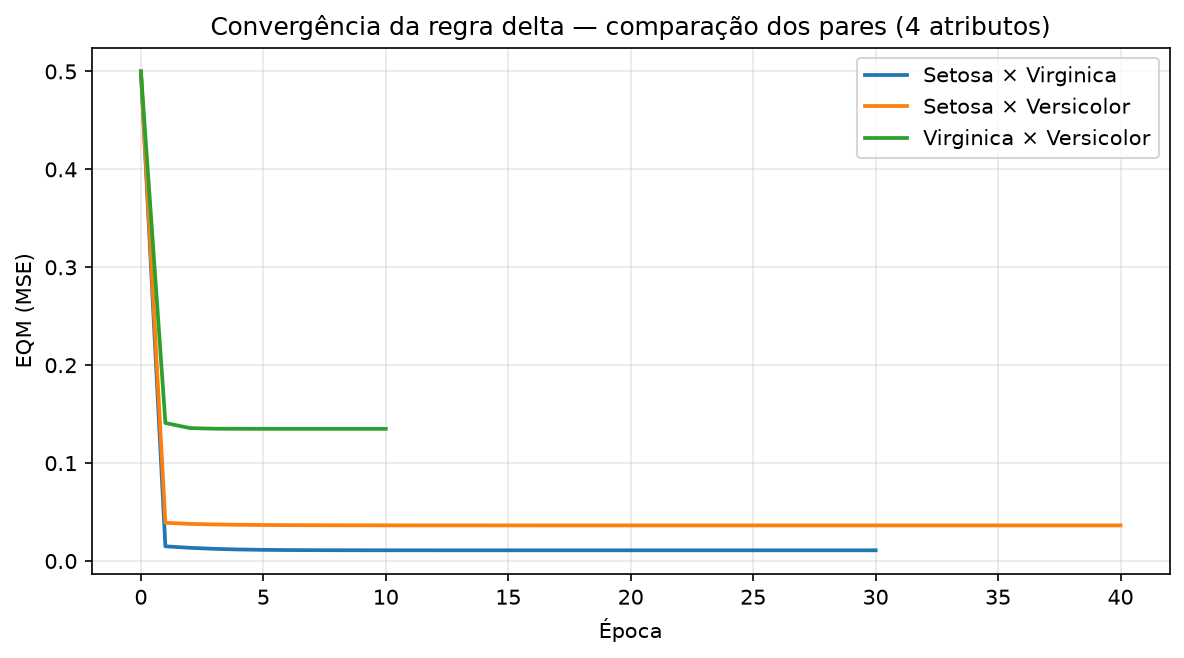
\includegraphics[width=0.85\textwidth]{figuras/mse_iris_comparacao.png}
\caption{EQM por época nos três pares da Iris com os quatro atributos.}
\label{fig:mse_iris}
\end{figure}

Com apenas os dois atributos da sépala, os pares com a \setosa{} continuam linearmente separáveis no treinamento (o perceptron simples encontra uma reta sem erros), mas a solução de EQM mínimo da regra delta deixa 3 e 2 padrões do lado errado. É a ilustração direta da Seção~\ref{sec:regra_delta}: a regra delta minimiza o erro quadrático, e os padrões distantes da fronteira também puxam a solução, que nem sempre coincide com uma reta separadora. No par \virginica{}~$\times$~\versicolor{}, a sobreposição na sépala é grande e o acerto no teste cai para 73,33\% (Figura~\ref{fig:dispersao}).

\begin{figure}[H]
\centering
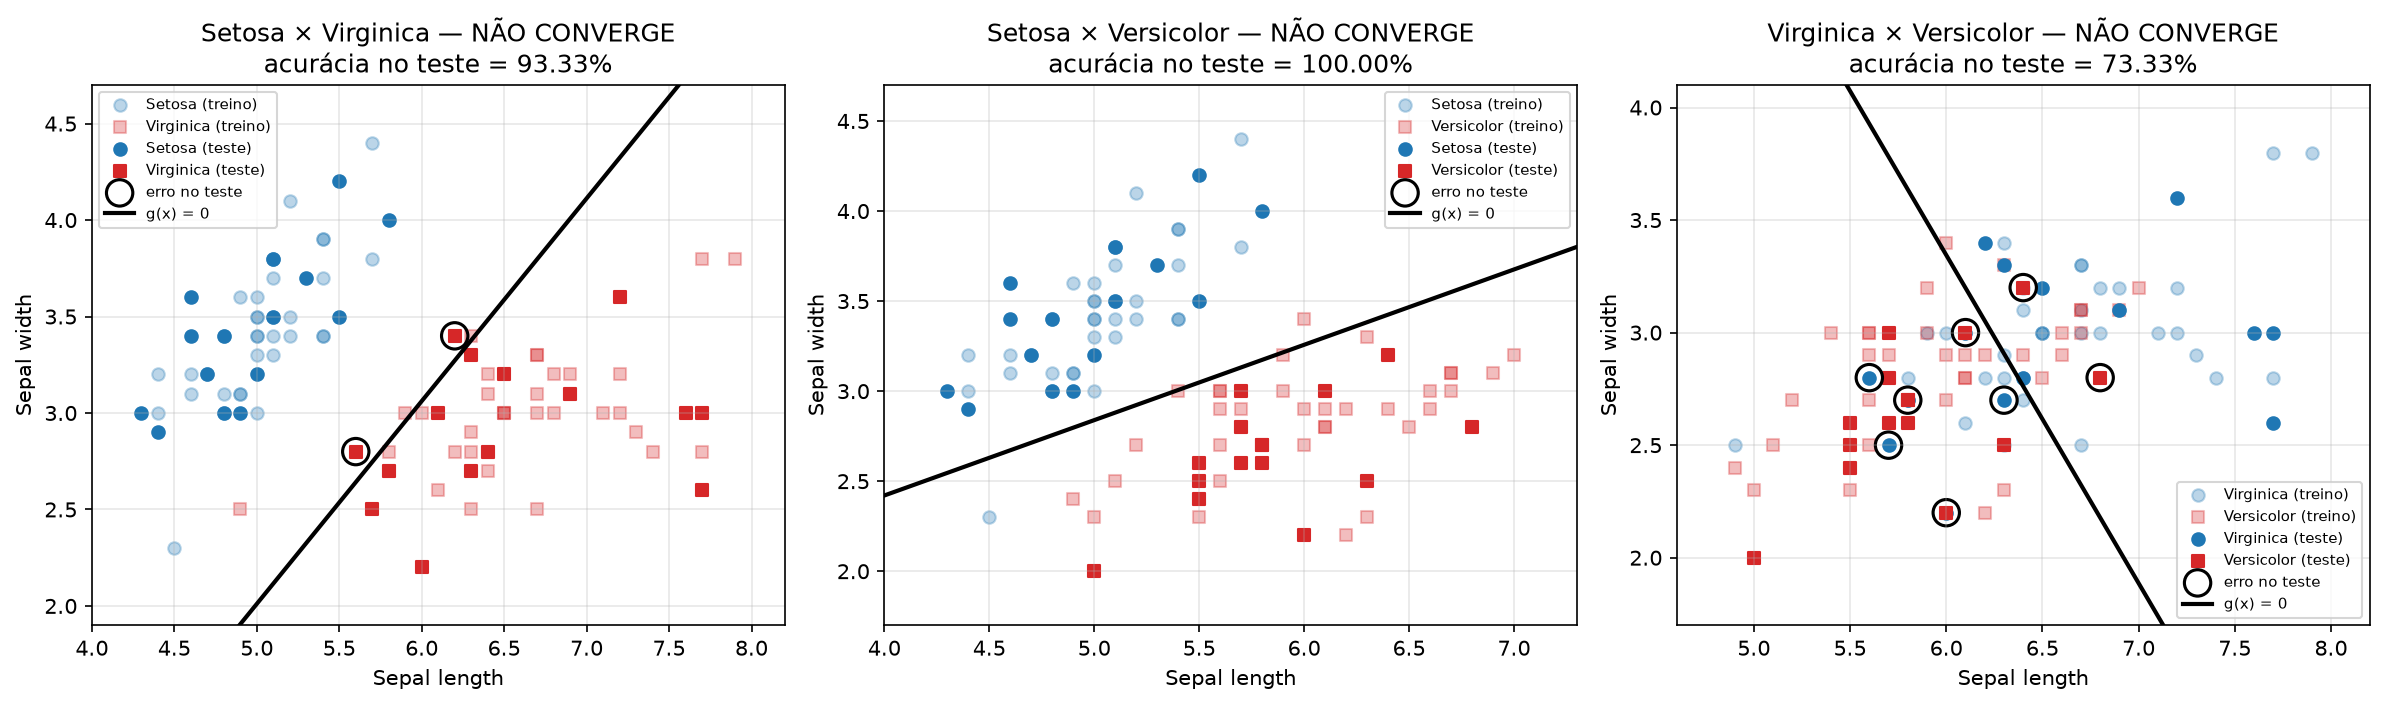
\includegraphics[width=\textwidth]{figuras/dispersao_iris_2d.png}
\caption{Dispersão do conjunto de teste nos dois atributos da sépala e retas obtidas pela regra delta.}
\label{fig:dispersao}
\end{figure}

\subsection{Tabelas verdade}

Com as saídas 1 e 0 mapeadas para $+1$ e $-1$, a regra delta classificou corretamente os quatro padrões de OR e AND (Figura~\ref{fig:tabelas}). O EQM final (0,1289) ficou um pouco acima do mínimo de mínimos quadrados (0,125): com $\alpha$ constante e correção a cada padrão, os pesos oscilam em torno do mínimo. No XOR, a melhor solução linear é $\mathbf{w} = \mathbf{0}$, com EQM $= 0{,}5$, em que $g(\mathbf{x}) = 0$ para todas as entradas. A regra delta termina perto dela, com $\mathbf{w} = (0{,}25;\ 0;\ 0)^t$, EQM $= 0{,}5156$ e dois acertos em quatro: nenhuma reta separa o XOR, que exige uma camada intermediária de perceptrons.

\begin{figure}[H]
\centering
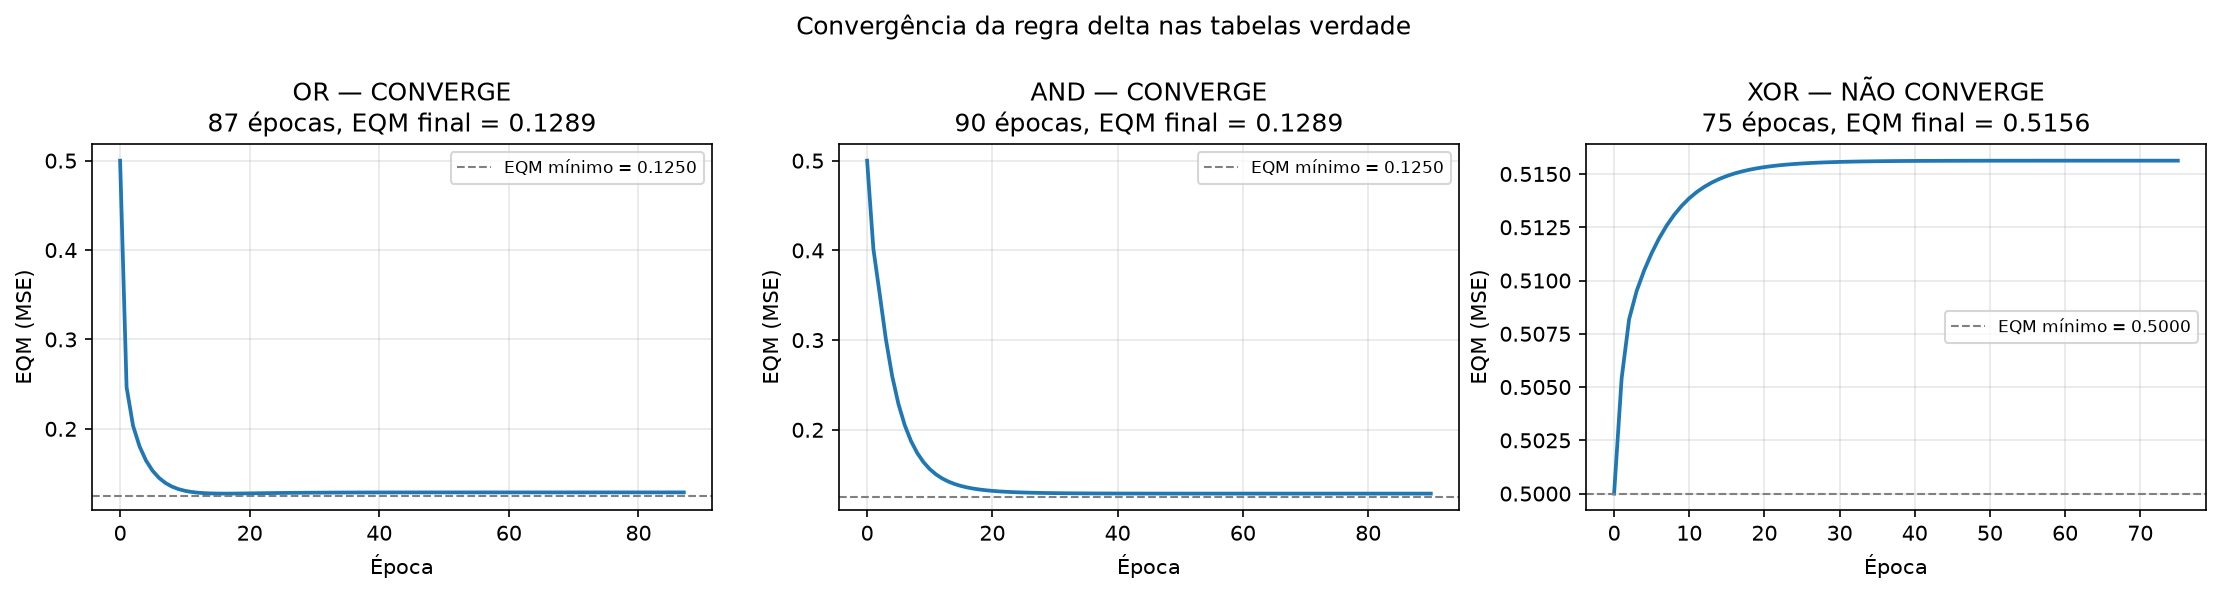
\includegraphics[width=0.49\textwidth]{figuras/mse_tabelas_verdade.png}\hfill
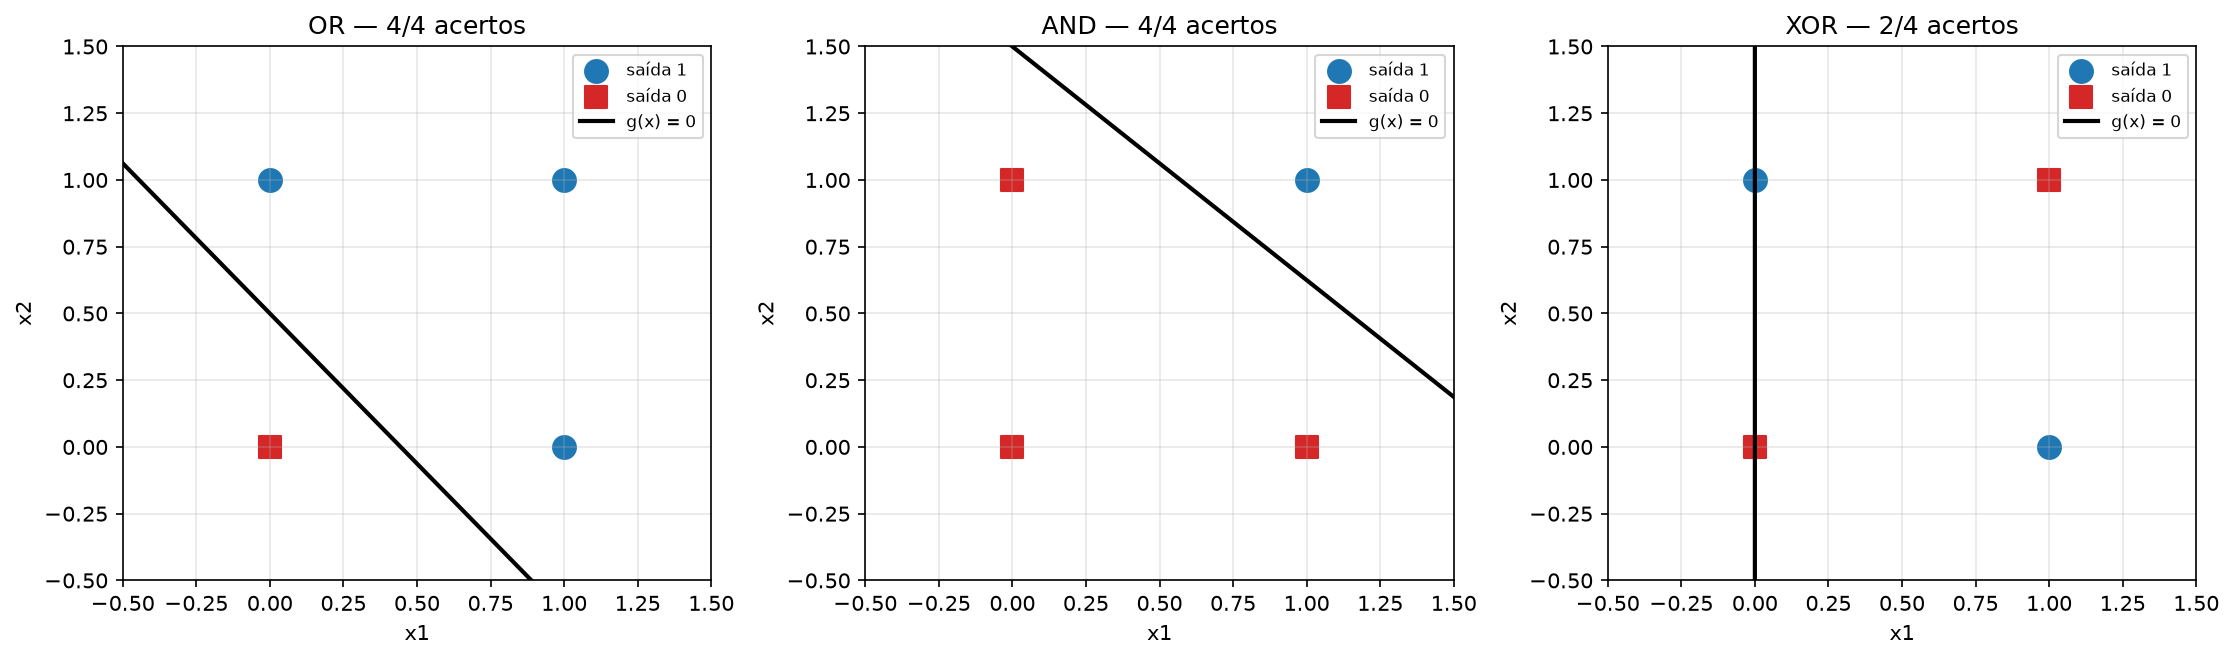
\includegraphics[width=0.49\textwidth]{figuras/fronteiras_tabelas_verdade.png}
\caption{Tabelas verdade: EQM por época (esquerda) e retas de decisão (direita).}
\label{fig:tabelas}
\end{figure}

%=====================================================================
\section{Parte II --- Comparação dos classificadores pelas métricas de qualidade}\label{sec:parte2}
%=====================================================================

Todas as métricas desta seção foram calculadas no conjunto de teste (45 amostras, 15 de cada espécie), com os quatro atributos.

\subsection{Matrizes de confusão}

A Figura~\ref{fig:matrizes} mostra as cinco matrizes. A \setosa{} é classificada sem erro por todos os métodos, e todos os erros estão entre \versicolor{} e \virginica{}. As matrizes da distância mínima e do máximo da função de decisão são idênticas, como previsto na Seção~\ref{sec:classificadores}.

\begin{figure}[H]
\centering
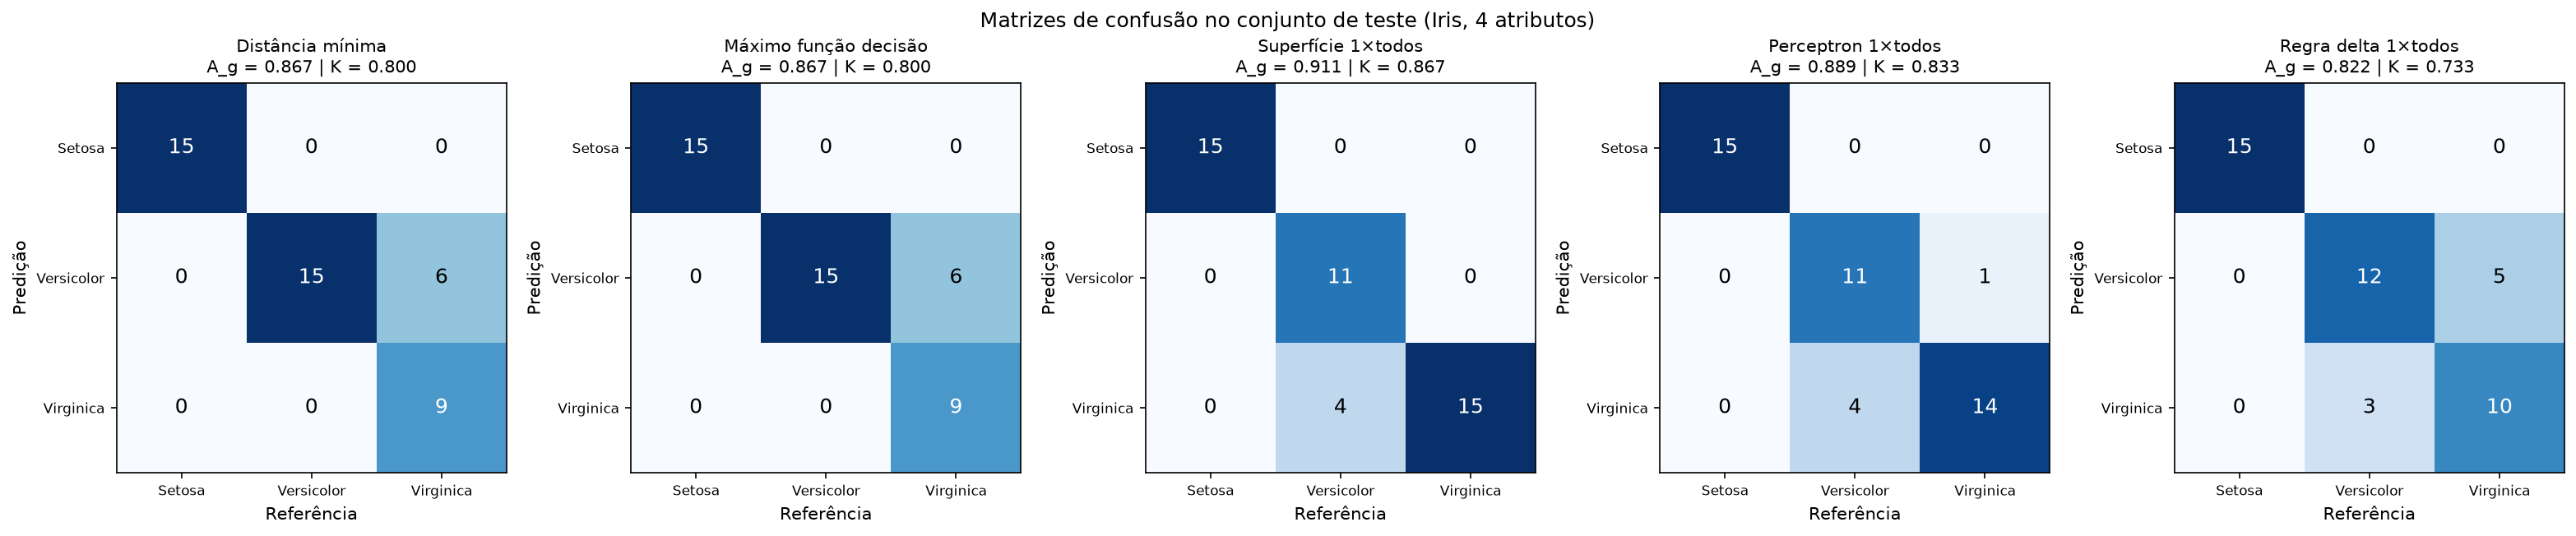
\includegraphics[width=\textwidth]{figuras/matrizes_confusao.png}
\caption{Matrizes de confusão no conjunto de teste (linhas: predição; colunas: referência).}
\label{fig:matrizes}
\end{figure}

Treinados na estratégia um contra todos, os perceptrons de \versicolor{} $\times$ resto e \virginica{} $\times$ resto não convergiram em 1000 épocas, pois essas classes não são linearmente separáveis do resto; o de \setosa{} convergiu em 2 épocas. Na regra delta, o EQM estabilizou nas três classes, em 24, 29 e 27 épocas.

\subsection{Questão 1 --- métricas multiclasse}

\begin{table}[H]
\centering
\caption{Acerto global, Kappa e Tau com as respectivas variâncias (teste, $m = 45$, $C = 3$).}
\label{tab:multiclasse}
\small
\begin{tabular}{lcccccl}
\toprule
Classificador & $A_g$ & $K$ & $\sigma_K^2$ & $\tau$ & $\sigma_\tau^2$ & Concordância \\
\midrule
Distância mínima            & 0,8667 & 0,8000 & 0,005446 & 0,8000 & 0,005778 & substancial \\
Máximo da função de decisão & 0,8667 & 0,8000 & 0,005446 & 0,8000 & 0,005778 & substancial \\
Superfície um contra todos  & 0,9111 & 0,8667 & 0,003949 & 0,8667 & 0,004049 & quase perfeita \\
Perceptron um contra todos  & 0,8889 & 0,8333 & 0,004868 & 0,8333 & 0,004938 & quase perfeita \\
Regra delta um contra todos & 0,8222 & 0,7333 & 0,007261 & 0,7333 & 0,007309 & substancial \\
\bottomrule
\end{tabular}
\end{table}

\begin{table}[H]
\centering
\caption{Acurácias do produtor ($A_p$) e do usuário ($A_u$) por classe.}
\label{tab:prod_usu}
\small
\begin{tabular}{lcccccc}
\toprule
 & \multicolumn{3}{c}{$A_p$ (sensibilidade)} & \multicolumn{3}{c}{$A_u$ (precisão)} \\
\cmidrule(lr){2-4}\cmidrule(lr){5-7}
Classificador & \setosa{} & \versicolor{} & \virginica{} & \setosa{} & \versicolor{} & \virginica{} \\
\midrule
Distância mínima            & 1,0000 & 1,0000 & 0,6000 & 1,0000 & 0,7143 & 1,0000 \\
Máximo da função de decisão & 1,0000 & 1,0000 & 0,6000 & 1,0000 & 0,7143 & 1,0000 \\
Superfície um contra todos  & 1,0000 & 0,7333 & 1,0000 & 1,0000 & 1,0000 & 0,7895 \\
Perceptron um contra todos  & 1,0000 & 0,7333 & 0,9333 & 1,0000 & 0,9167 & 0,7778 \\
Regra delta um contra todos & 1,0000 & 0,8000 & 0,6667 & 1,0000 & 0,7059 & 0,7692 \\
\bottomrule
\end{tabular}
\end{table}

As acurácias do produtor e do usuário mostram que os classificadores erram em direções opostas. A distância mínima (e o máximo da função de decisão) empurra \virginica{} para \versicolor{}: todas as \versicolor{} são reconhecidas ($A_p = 1$), mas só 60\% das \virginica{}, e 29\% do que é chamado de \versicolor{} é, na verdade, \virginica{} ($A_u = 0{,}71$). A superfície um contra todos e o perceptron fazem o contrário: perdem 4 das 15 \versicolor{} e reconhecem quase todas as \virginica{}. A regra delta divide os erros entre as duas classes e tem o menor acerto global.

\paragraph{Kappa igual a Tau.} Em todos os classificadores, $K = \tau$. Não é coincidência: como o conjunto de teste é balanceado, $a_{+i} = m/C$ para toda classe, e o acerto casual da Eq.~\eqref{eq:kappa} se torna
\begin{equation}
  A_a = \frac{1}{m^2}\sum_{i=1}^{C} a_{i+}\,\frac{m}{C} = \frac{1}{mC}\sum_{i=1}^{C} a_{i+} = \frac{1}{C},
\end{equation}
que é exatamente a hipótese do Tau. As variâncias, porém, diferem, porque a do Kappa depende da distribuição das predições ($a_{i+}$) e a do Tau, não.

\subsection{Questão 1 --- problema de duas classes}

\begin{table}[H]
\centering
\caption{Métricas binárias ``classe $\times$ resto'' no conjunto de teste.}
\label{tab:binarias}
\footnotesize
\setlength{\tabcolsep}{4pt}
\begin{tabular}{llrrrrcccccc}
\toprule
Classificador & Classe & VP & FP & FN & VN & Sens. & Espec. & Prec. & $F_1$ & $F_2$ & MCC \\
\midrule
\multirow{3}{*}{Dist. mín. / Máximo}
 & \setosa{}     & 15 & 0 & 0 & 30 & 1,000 & 1,000 & 1,000 & 1,000 & 1,000 & 1,000 \\
 & \versicolor{} & 15 & 6 & 0 & 24 & 1,000 & 0,800 & 0,714 & 0,833 & 0,926 & 0,756 \\
 & \virginica{}  & 9  & 0 & 6 & 30 & 0,600 & 1,000 & 1,000 & 0,750 & 0,652 & 0,707 \\
\midrule
\multirow{3}{*}{Superfície 1$\times$todos}
 & \setosa{}     & 15 & 0 & 0 & 30 & 1,000 & 1,000 & 1,000 & 1,000 & 1,000 & 1,000 \\
 & \versicolor{} & 11 & 0 & 4 & 30 & 0,733 & 1,000 & 1,000 & 0,846 & 0,775 & 0,804 \\
 & \virginica{}  & 15 & 4 & 0 & 26 & 1,000 & 0,867 & 0,789 & 0,882 & 0,949 & 0,827 \\
\midrule
\multirow{3}{*}{Perceptron 1$\times$todos}
 & \setosa{}     & 15 & 0 & 0 & 30 & 1,000 & 1,000 & 1,000 & 1,000 & 1,000 & 1,000 \\
 & \versicolor{} & 11 & 1 & 4 & 29 & 0,733 & 0,967 & 0,917 & 0,815 & 0,764 & 0,746 \\
 & \virginica{}  & 14 & 4 & 1 & 26 & 0,933 & 0,867 & 0,778 & 0,848 & 0,897 & 0,770 \\
\midrule
\multirow{3}{*}{Regra delta 1$\times$todos}
 & \setosa{}     & 15 & 0 & 0 & 30 & 1,000 & 1,000 & 1,000 & 1,000 & 1,000 & 1,000 \\
 & \versicolor{} & 12 & 5 & 3 & 25 & 0,800 & 0,833 & 0,706 & 0,750 & 0,779 & 0,616 \\
 & \virginica{}  & 10 & 3 & 5 & 27 & 0,667 & 0,900 & 0,769 & 0,714 & 0,685 & 0,589 \\
\bottomrule
\end{tabular}
\end{table}

\begin{table}[H]
\centering
\caption{Médias de $F_1$, $F_2$ e MCC sobre as três classes.}
\label{tab:medias}
\begin{tabular}{lccc}
\toprule
Classificador & $F_1$ & $F_2$ & MCC \\
\midrule
Distância mínima / Máximo   & 0,8611 & 0,8594 & 0,8210 \\
Superfície um contra todos  & 0,9095 & 0,9080 & 0,8772 \\
Perceptron um contra todos  & 0,8878 & 0,8871 & 0,8387 \\
Regra delta um contra todos & 0,8214 & 0,8214 & 0,7351 \\
\bottomrule
\end{tabular}
\end{table}

O ranking pelas médias de $F_1$ e MCC é o mesmo do Kappa. O MCC é a medida mais severa, porque usa os quatro valores da matriz: os da regra delta para \versicolor{} e \virginica{} (0,62 e 0,59) ficam bem abaixo dos $F_1$ correspondentes (0,75 e 0,71). O $F_2$ deixa visível o peso da sensibilidade: na distância mínima, \versicolor{} (sensibilidade 1) sobe de $F_1 = 0{,}833$ para $F_2 = 0{,}926$, e \virginica{} (sensibilidade 0,60) cai de 0,750 para 0,652.

\subsection{Questão 2 --- testes de significância}

\begin{table}[H]
\centering
\caption{Testes de significância pedidos ($\alpha = 5\%$, $Z_{0{,}975} = 1{,}96$).}
\label{tab:testes}
\begin{tabular}{llcccc}
\toprule
Comparação & Coef. & $k_1$ & $k_2$ & $Z$ & p-valor \\
\midrule
Superfície 1$\times$todos vs.\ perceptron   & Kappa & 0,8667 & 0,8333 & $+0{,}355$ & 0,723 \\
Regra delta vs.\ perceptron                 & Kappa & 0,7333 & 0,8333 & $-0{,}908$ & 0,364 \\
Regra delta vs.\ perceptron                 & Tau   & 0,7333 & 0,8333 & $-0{,}904$ & 0,366 \\
\bottomrule
\end{tabular}
\end{table}

\paragraph{Superfície de decisão vs.\ perceptron.} A superfície um contra todos tem Kappa um pouco maior (0,867 contra 0,833), mas $|Z| = 0{,}36 < 1{,}96$ e $p = 0{,}72$: não se rejeita $H_0$, e os dois classificadores não diferem significativamente ao nível de 5\%. Se houvesse diferença significativa, ela significaria que a concordância de um dos classificadores com a referência é maior do que a do outro além do que a variação da amostra de teste explica, ou seja, que um deles é de fato melhor para esse problema, e não apenas nessa amostra.

\paragraph{Regra delta vs.\ perceptron.} O perceptron tem maior acurácia ($A_g = 0{,}889$ contra 0,822) e maiores Kappa e Tau, mas os testes dão $Z = -0{,}91$ ($p = 0{,}36$) para o Kappa e $Z = -0{,}90$ ($p = 0{,}37$) para o Tau. Em nenhum dos dois casos se rejeita $H_0$. O p-valor diz que, se os dois classificadores fossem equivalentes, uma diferença de Kappa pelo menos desse tamanho apareceria por acaso em cerca de 36\% das amostras de teste: não há evidência de que o perceptron seja melhor.

\paragraph{Todos os pares.} A Tabela~\ref{tab:z_todos} mostra que nenhum par de classificadores difere a 5\%; o maior $|Z|$ é 1,26, entre a superfície e a regra delta. O motivo é o tamanho da amostra: com $m = 45$, $\sigma_K \approx 0{,}07$, e uma diferença de Kappa só seria significativa a partir de cerca de $1{,}96\sqrt{2 \times 0{,}005} \approx 0{,}2$.

\begin{table}[H]
\centering
\caption{Estatística $Z$ do Kappa entre todos os pares (linha menos coluna).}
\label{tab:z_todos}
\small
\begin{tabular}{lccccc}
\toprule
 & Dist. mín. & Máximo & Superfície & Perceptron & Regra delta \\
\midrule
Distância mínima  & ---      & 0,000    & $-0{,}688$ & $-0{,}328$ & $+0{,}591$ \\
Máximo            & 0,000    & ---      & $-0{,}688$ & $-0{,}328$ & $+0{,}591$ \\
Superfície        & $+0{,}688$ & $+0{,}688$ & ---      & $+0{,}355$ & $+1{,}259$ \\
Perceptron        & $+0{,}328$ & $+0{,}328$ & $-0{,}355$ & ---      & $+0{,}908$ \\
Regra delta       & $-0{,}591$ & $-0{,}591$ & $-1{,}259$ & $-0{,}908$ & ---      \\
\bottomrule
\end{tabular}
\end{table}

%=====================================================================
\section{Parte III --- Exercícios da aula PR51}\label{sec:parte3}
%=====================================================================

As matrizes seguem a mesma convenção (linhas: predição; colunas: referência).

\subsection{Teste RT-PCR para COVID-19}

Com VP $= 185$, FP $= 30$, FN $= 15$ e VN $= 770$, a acurácia confere com a aula (95,5\%). A sensibilidade é 0,925, a especificidade 0,9625, a precisão 0,8605, $F_1 = 0{,}892$, $F_2 = 0{,}911$, MCC $= 0{,}864$ e $K = 0{,}863$ (quase perfeita). Os 15 infectados com resultado negativo são o erro mais grave numa doença transmissível.

\subsection{Concordância entre radiologistas}

\begin{table}[H]
\centering
\caption{Mamografias classificadas por dois radiologistas.}
\label{tab:radiologistas}
\begin{tabular}{lccc}
\toprule
Rad. A $\backslash$ Rad. B & Normal & Benigno & Maligno \\
\midrule
Normal  & 88 & 5  & 2  \\
Benigno & 8  & 52 & 4  \\
Maligno & 3  & 6  & 32 \\
\bottomrule
\end{tabular}
\end{table}

Com $m = 200$, $A_g = 0{,}86$ e $A_a = 0{,}3749$, obtém-se $K = 0{,}776$ (concordância substancial), com $\sigma_K^2 = 0{,}001512$, conferindo o valor de 0,78 da aula. O teste $Z = K/\sigma_K = 19{,}96$ mostra que essa concordância é muito superior à do acaso. O Tau ($\tau = 0{,}79$, $\sigma_\tau^2 = 0{,}001355$) é um pouco maior que o Kappa porque supõe acerto casual de $1/3$, enquanto as marginais reais concentram casos em ``Normal'' ($A_a = 0{,}375 > 1/3$).

\subsection{Rastreamento de câncer de mama}

A tabela da aula é inconsistente: $90 + 495 + 10 + 9\,415 = 10\,010$, e a coluna ``Saudável'' soma 9\,910, e não 9\,900. Mantendo os totais do enunciado (100 casos, 9\,900 saudáveis, 10\,000 no total), foi usado VN $= 9\,900 - 495 = 9\,405$.

A acurácia é de 94,95\%, a sensibilidade 0,90 e a especificidade 0,95, mas a precisão é só 0,154: com prevalência de 1\%, a mamografia gera cinco vezes mais falsos positivos que verdadeiros positivos. Um classificador que dissesse ``saudável'' para todas teria 99\% de acurácia e sensibilidade nula. As demais métricas mostram o problema: $F_1 = 0{,}263$, MCC $= 0{,}360$ e $K = 0{,}250$. O $F_2 = 0{,}457$ é maior que o $F_1$ porque valoriza a sensibilidade de 90\%, que é o que importa num rastreamento.

\subsection{Desafio obrigatório: classificadores A e B}\label{sec:desafio}

\begin{table}[H]
\centering
\caption{Matrizes de confusão dos classificadores A ($m = 610$) e B ($m = 620$).}
\label{tab:desafio_mc}
\begin{tabular}{l|cccc||l|cccc}
\toprule
A & $\omega_1$ & $\omega_2$ & $\omega_3$ & $\omega_4$ & B & $\omega_1$ & $\omega_2$ & $\omega_3$ & $\omega_4$ \\
\midrule
$\omega_1$ & 140 & 20  & 0   & 0   & $\omega_1$ & 140 & 30  & 2   & 0   \\
$\omega_2$ & 10  & 130 & 0   & 0   & $\omega_2$ & 10  & 110 & 5   & 0   \\
$\omega_3$ & 5   & 0   & 150 & 10  & $\omega_3$ & 0   & 10  & 140 & 0   \\
$\omega_4$ & 15  & 10  & 0   & 120 & $\omega_4$ & 20  & 10  & 3   & 140 \\
\bottomrule
\end{tabular}
\end{table}

\begin{table}[H]
\centering
\caption{Métricas dos classificadores A e B.}
\label{tab:desafio_metricas}
\small
\begin{tabular}{lcc}
\toprule
 & A & B \\
\midrule
$A_g$          & 0,8852 & 0,8548 \\
$A_a$          & 0,2505 & 0,2496 \\
$A_p$ ($\omega_1$, $\omega_2$, $\omega_3$, $\omega_4$) & 0,824; 0,813; 1,000; 0,923 & 0,824; 0,688; 0,933; 1,000 \\
$A_u$ ($\omega_1$, $\omega_2$, $\omega_3$, $\omega_4$) & 0,875; 0,929; 0,909; 0,828 & 0,814; 0,880; 0,933; 0,809 \\
Kappa $K$      & 0,8469 & 0,8065 \\
$\sigma_K^2$   & 0,000295 & 0,000353 \\
Tau $\tau$     & 0,8470 & 0,8065 \\
$\sigma_\tau^2$ & 0,000296 & 0,000356 \\
\bottomrule
\end{tabular}
\end{table}

\paragraph{Teste com o Kappa.} $Z = (0{,}8469 - 0{,}8065)/\sqrt{0{,}000295 + 0{,}000353} = 1{,}585$. Como $|Z| < 1{,}96$, não se rejeita $H_0$: ao nível de 5\%, os dois modelos não diferem. O p-valor é 0,113: se os modelos fossem equivalentes, uma diferença de Kappa pelo menos desse tamanho apareceria por acaso em cerca de 11\% das amostras. É pouco provável, mas não o bastante para o nível adotado; a diferença só seria significativa para $\alpha > 0{,}113$.

\paragraph{Teste com o Tau.} $Z = 1{,}588$ e $p = 0{,}112$; a conclusão é a mesma. Kappa e Tau ficam muito próximos porque as marginais da referência são quase uniformes, o que leva $A_a \approx 0{,}25 = 1/C$.

\subsection{Caso clínico: diabetes tipo 2}

\begin{table}[H]
\centering
\caption{Matriz de confusão do modelo de triagem de diabetes.}
\label{tab:diabetes}
\begin{tabular}{lccc}
\toprule
 & Diabetes (real) & Saudável (real) & Total \\
\midrule
Positivo & 255 & 120  & 375  \\
Negativo & 45  & 1\,580 & 1\,625 \\
Total    & 300 & 1\,700 & 2\,000 \\
\bottomrule
\end{tabular}
\end{table}

\begin{enumerate}
  \item Acurácia $= 0{,}9175$, sensibilidade $= 0{,}85$, especificidade $= 0{,}9294$, precisão $= 0{,}68$, $F_1 = 0{,}7556$ ($F_2 = 0{,}8095$, MCC $= 0{,}713$, $K = 0{,}707$).
  \item Na triagem inicial deve-se priorizar a \textbf{sensibilidade} (ou o $F_2$): o objetivo é não deixar diabéticos sem diagnóstico. Um falso positivo gera apenas um exame confirmatório barato (glicemia de jejum, HbA1c), enquanto um falso negativo deixa a doença evoluir sem tratamento.
  \item Os 45 falsos negativos (15\% dos diabéticos) saem da triagem achando que estão saudáveis. O risco clínico é a progressão silenciosa da doença e de suas complicações (retinopatia, nefropatia, neuropatia, doença cardiovascular) e o atraso no tratamento. A métrica afetada é a sensibilidade, e com ela o $F_1$ e o $F_2$.
  \item Não. Aplicando a mesma sensibilidade e especificidade a 2\,000 pacientes com prevalência de 5\%, a acurácia passa a 92,5\% sem nenhuma mudança no modelo, e um classificador trivial que nunca acusa diabetes teria 95\%. A precisão cai de 0,68 para 0,39 ($F_1 = 0{,}53$, MCC $= 0{,}54$). Para comparar populações com prevalências diferentes devem-se usar sensibilidade e especificidade, que não dependem da prevalência, e o MCC, que resume a matriz inteira.
  \item Não. Kappa $= 0{,}65$ indica concordância substancial, mas entre os \emph{dois endocrinologistas}, e não entre o modelo e a referência. Ele mostra que o próprio padrão-ouro tem variabilidade. Para validar o modelo é preciso calcular o Kappa do modelo contra essa referência (ou contra cada especialista) e verificar se ele é comparável ao Kappa entre os especialistas. Além disso, com 100 casos a variância do Kappa é grande.
\end{enumerate}

\subsection{Caso clínico: pneumonia em raio-X}

\begin{table}[H]
\centering
\caption{Métricas de cada avaliador contra o laudo de referência (5\,000 imagens, prevalência de 20\%).}
\label{tab:pneumonia}
\small
\begin{tabular}{lrrrrcccccc}
\toprule
Avaliador & VP & FP & FN & VN & Sens. & Espec. & Prec. & $F_1$ & MCC & $K$ \\
\midrule
Modelo de IA   & 920 & 280 & 80  & 3\,720 & 0,920 & 0,930 & 0,767 & 0,836 & 0,796 & 0,791 \\
Radiologista A & 940 & 150 & 60  & 3\,850 & 0,940 & 0,963 & 0,862 & 0,900 & 0,874 & 0,873 \\
Radiologista B & 890 & 100 & 110 & 3\,900 & 0,890 & 0,975 & 0,899 & 0,895 & 0,868 & 0,868 \\
\bottomrule
\end{tabular}
\end{table}

\begin{enumerate}
  \item Os valores estão na Tabela~\ref{tab:pneumonia}.
  \item A IA não supera o Radiologista A em nenhuma métrica. Ela supera o Radiologista B em \textbf{sensibilidade} (0,920 contra 0,890): deixa de detectar 80 pneumonias, contra 110. Em compensação, tem quase três vezes mais falsos positivos (280 contra 100) e perde em especificidade, precisão, $F_1$ e MCC. A IA está calibrada para não perder casos, o comportamento desejado numa segunda leitura.
  \item O enunciado dá apenas a matriz de cada avaliador contra a referência. O Kappa \emph{entre} dois avaliadores exige a tabela cruzada (quantas imagens a IA e o Rad. A laudaram igual e diferente), que não pode ser reconstruída a partir das matrizes individuais. O que se pode calcular é o Kappa de cada um contra a referência: IA $= 0{,}791$, Rad. A $= 0{,}873$ e Rad. B $= 0{,}868$. Pelo teste $Z$, a IA concorda significativamente menos com a referência que o Rad. A ($Z = -6{,}08$) e que o Rad. B ($Z = -5{,}64$), enquanto os dois radiologistas não diferem entre si ($Z = 0{,}39$, $p = 0{,}70$).
  \item Um critério razoável para aprovar a IA como segunda leitura é Kappa (IA $\times$ médico) $\ge 0{,}61$, ou seja, concordância pelo menos substancial, e, de forma mais rigorosa, que esse Kappa não seja significativamente menor que o Kappa entre os próprios radiologistas (teste $Z$ com $p > 0{,}05$). Contra a referência, a IA atende ao primeiro critério ($K = 0{,}79$), mas não ao segundo.
  \item Com prevalência de 5\% e a mesma sensibilidade e especificidade, o VPP da IA cai de 0,767 para 0,409: a maioria dos positivos passa a ser alarme falso, porque os negativos são muito mais numerosos. O $F_1$ cai de 0,836 para 0,566 e o MCC, de 0,796 para 0,586. O MCC é a métrica mais útil nesse cenário: o $F_1$ ignora os VN e muda se a classe ``positiva'' for trocada, enquanto o MCC usa os quatro valores da matriz, é simétrico entre as classes e só se aproxima de 1 quando o classificador acerta bem as duas~\cite{chicco}.
\end{enumerate}

\begin{table}[H]
\centering
\caption{Efeito da queda da prevalência de 20\% para 5\% (mesma sensibilidade e especificidade).}
\label{tab:prevalencia}
\begin{tabular}{lcccccc}
\toprule
 & \multicolumn{2}{c}{VPP} & \multicolumn{2}{c}{$F_1$} & \multicolumn{2}{c}{MCC} \\
\cmidrule(lr){2-3}\cmidrule(lr){4-5}\cmidrule(lr){6-7}
Avaliador & 20\% & 5\% & 20\% & 5\% & 20\% & 5\% \\
\midrule
Modelo de IA   & 0,767 & 0,409 & 0,836 & 0,566 & 0,796 & 0,586 \\
Radiologista A & 0,862 & 0,569 & 0,900 & 0,709 & 0,874 & 0,714 \\
Radiologista B & 0,899 & 0,652 & 0,895 & 0,753 & 0,868 & 0,748 \\
\bottomrule
\end{tabular}
\end{table}

%=====================================================================
\section{Discussão}
%=====================================================================

A regra delta se comportou como a teoria prevê: o EQM estabilizou em todos os problemas, separáveis ou não, mas a separação sem erros só foi obtida quando as classes eram linearmente separáveis e, mesmo assim, nem sempre. Com os dois atributos da sépala, os pares com a \setosa{} são separáveis e ainda assim a solução de EQM mínimo deixou padrões do lado errado. Essa é a principal diferença em relação ao perceptron simples, que só para quando todos os padrões estão corretos e, em compensação, não para quando as classes não são separáveis.

A mesma diferença aparece na comparação das três classes. Com as classes \versicolor{} e \virginica{} não separáveis do resto, o perceptron simples terminou em 1000 épocas com os pesos da última correção, e seu desempenho depende de onde o treinamento foi interrompido. A regra delta converge sempre, mas minimiza o erro quadrático e não o número de erros, e neste teste ficou com o menor acerto global. A superfície de decisão um contra todos, que usa apenas as médias das classes, obteve os melhores valores de todas as métricas.

As métricas da PR51 acrescentam informação que a acurácia sozinha não dá. As acurácias do produtor e do usuário revelam que a distância mínima e a superfície de decisão erram em direções opostas, ainda que com acurácias próximas. O MCC é mais severo que o $F_1$ porque considera os VN, e o $F_2$ evidencia os classificadores que privilegiam a sensibilidade. Nos exercícios clínicos, ficou claro que a acurácia é enganosa quando a prevalência é baixa: no rastreamento de câncer de mama, 95\% de acurácia convivem com precisão de 15\%.

O teste de significância muda a leitura dos resultados. Os cinco classificadores têm Kappas entre 0,73 e 0,87, mas nenhuma diferença é significativa a 5\%. Com apenas 45 amostras de teste, cada erro altera o acerto global em 2,2 pontos percentuais, e o desvio padrão do Kappa fica em torno de 0,07. No desafio da aula, com mais de 600 amostras por classificador, as variâncias são cerca de 15 vezes menores, mas uma diferença de 0,04 no Kappa ainda não é suficiente para rejeitar $H_0$.

Algumas limitações devem ser registradas. Os resultados vêm de uma única divisão 70/30 com semente fixa; outra divisão poderia mudar a ordem dos classificadores, que de qualquer forma não diferem estatisticamente. O teste $Z$ supõe que as duas matrizes sejam independentes, mas na Parte II os cinco classificadores foram avaliados nas mesmas 45 amostras, o que torna o teste conservador. Por fim, na estratégia um contra todos, os classificadores binários são treinados com classes desbalanceadas (35 amostras contra 70).

%=====================================================================
\section{Conclusão}
%=====================================================================

O perceptron com regra delta foi implementado sem bibliotecas de aprendizado de máquina e aplicado aos pares da Iris e às tabelas verdade. O EQM convergiu em todos os casos; a separação sem erros foi obtida nos pares com a \setosa{} (quatro atributos) e nas tabelas OR e AND, mas não no par \virginica{}~$\times$~\versicolor{} nem no XOR, que não são linearmente separáveis.

As métricas de qualidade da aula PR51 foram implementadas e validadas com os exemplos dos slides e por simulação, e usadas para comparar cinco classificadores das três classes da Iris. A superfície de decisão um contra todos obteve os maiores acerto global (0,911), Kappa e Tau (0,867) e MCC médio (0,877), seguida do perceptron, da distância mínima (idêntica ao máximo da função de decisão) e da regra delta. No conjunto de teste balanceado, Kappa e Tau coincidiram, como mostrado algebricamente.

Pelos testes de significância, a superfície de decisão e o perceptron não diferem quanto ao Kappa ($Z = 0{,}36$, $p = 0{,}72$), e a regra delta e o perceptron também não diferem, nem pelo Kappa ($Z = -0{,}91$, $p = 0{,}36$) nem pelo Tau ($Z = -0{,}90$, $p = 0{,}37$). A maior acurácia do perceptron em relação à regra delta, portanto, não é estatisticamente significativa ao nível de 5\%. No desafio obrigatório da aula, os classificadores A e B também não diferem ($Z = 1{,}59$, $p = 0{,}11$ para o Kappa e para o Tau).

%=====================================================================
% Referências
%=====================================================================
\begin{thebibliography}{9}

\bibitem{sousa41}
SOUSA, R. P. de. \textbf{Perceptron: regra delta}. Material didático da disciplina Tópicos Especiais em Inteligência Artificial (PR41). Campina Grande: Universidade Estadual da Paraíba, 2026.

\bibitem{sousa51}
SOUSA, R. P. de. \textbf{Métricas de qualidade: machine learning --- aplicações em saúde e diagnóstico clínico}. Material didático da disciplina Tópicos Especiais em Inteligência Artificial (PR51). Campina Grande: Universidade Estadual da Paraíba, 2026.

\bibitem{congalton}
CONGALTON, R. G.; GREEN, K. \textbf{Assessing the Accuracy of Remotely Sensed Data: Principles and Practices}. 2. ed. Boca Raton: CRC Press, 2009.

\bibitem{landis}
LANDIS, J. R.; KOCH, G. G. The measurement of observer agreement for categorical data. \textbf{Biometrics}, v. 33, n. 1, p. 159--174, 1977.

\bibitem{chicco}
CHICCO, D.; JURMAN, G. The advantages of the Matthews correlation coefficient (MCC) over F1 score and accuracy in binary classification evaluation. \textbf{BMC Genomics}, v. 21, n. 1, p. 6, 2020.

\bibitem{sokolova}
SOKOLOVA, M.; LAPALME, G. A systematic analysis of performance measures for classification tasks. \textbf{Information Processing \& Management}, v. 45, n. 4, p. 427--437, 2009.

\bibitem{gonzalez}
GONZALEZ, R. C.; WOODS, R. E. \textbf{Digital Image Processing}. 4. ed. New York: Pearson, 2018.

\bibitem{repo}
PAMPLONA, J. \textbf{Laboratório 03: perceptron com regra delta e métricas de qualidade de classificadores}. Repositório de código-fonte, 2026. Disponível em: \repositorio. Acesso em: nov. 2026.

\end{thebibliography}

\end{document}
